% ******************************* Master Thesis Template **************************
% Please have a look at the README.txt file for info on how to use the template

\documentclass[a4paper,custommargin,times,numbered,langpt,printindex]{Classes/UCMScRProj}


% ******************************* Master Thesis Template **************************
% Please have a look at the README.txt file for info on how to use the template

\usepackage{amsmath}
\usepackage{amssymb}
\usepackage{amsthm}
\usepackage{enumitem}
\usepackage{graphicx}
\usepackage{comment}
\usepackage{hyperref}
\usepackage{booktabs}
\usepackage{xcolor,colortbl}
\definecolor{lavender}{rgb}{0.9, 0.9, 0.98}
%\usepackage{fancyhdr}
%\usepackage{acronym}
%\usepackage[default]{opensans}
%\usepackage{indentfirst}
%\setlength{\parindent}{1cm}
%\usepackage{setspace}
%\usepackage[avantgarde,nogrey]{quotchap}
\usepackage{xcolor}
%\usepackage[options]{subfigure}
%\usepackage[rightcaption]{sidecap}
%\usepackage{wrapfig}
\usepackage[portuguese]{babel}
\usepackage[utf8]{inputenc}
% ******************************************************************************
% ******************************* Class Options ********************************
% *********************** See README for more details **************************
% ******************************************************************************
% *********************** RECOMMENDATIONS **************************************

% `a4paper'
%
% `11pt'´(default): Font Size 12pt is NOT recommended.

% ********************** SOME OPTIONS ******************************************
%
% `oneside' or `twoside'(default): Printing double side (twoside) or single
% side.
%
% `print': Use `print' for print version with appropriate margins and page
% layout. Leaving the options field blank will activate Online version.
%
% `langen`: This redefines the style to English language if the MSc Thesis is written in English.
%  The default language is Portuguese. In this case of using Portuguese there is no need to declare it.
%
% `index': For index at the end of the thesis
%
% `draft': For draft mode without loading any images (same as draft in book)
%
% `draftmode': Special draft mode with line numbers, images, and water mark with
% timestamp and custom text. Position of the text can also be modified.
%
% `abstract': To generate only the title page and abstract page with
% dissertation title and name.
%
% `chapter`: This option enables only the specified chapter and it's references
%  Useful for review and corrections.
%
% ************************* Custom Page Margins ********************************
%
% `custommargin`: Use `custommargin' in options to activate custom page margins,
% which can be defined in the preamble.tex. Custom margin will override
% print/online margin setup.
%
% *********************** Choosing the Fonts in Class Options ******************
%
% `times' : Times font with math support.
%
% `fourier': Utopia Font with Fourier Math font (Font has to be installed)
%            It's a free font.
%
% `customfont': Use `customfont' option in the document class and load the
% package in the preamble.tex
%
% default or leave empty: `Latin Modern' font will be loaded.
%
% ********************** Choosing the Bibliography style ***********************
%
% `authoryear': For author-year citation eg., Krishna (2013)
%
% `numbered': (Default Option) For numbered and sorted citation e.g., [1,5,2]
%
% `custombib': Define your own bibliography style in the `preamble.tex' file.
%              `\RequirePackage[square, sort, numbers, authoryear]{natbib}'.
%              This can be also used to load biblatex instead of natbib
%              (See Preamble)
%
% **************************** Choosing the Page Style *************************
%
% `default (leave empty)': For Page Numbers in Header (Left Even, Right Odd) and
% Chapter Name in Header (Right Even) and Section Name (Left Odd). Blank Footer.
%
% `PageStyleI': Chapter Name next & Page Number on Even Side (Left Even).
% Section Name & Page Number in Header on Odd Side (Right Odd). Footer is empty.
%
% `PageStyleII': Chapter Name on Even Side (Left Even) in Header. Section Number
% and Section Name in Header on Odd Side (Right Odd). Page numbering in footer


% ********************************** Preamble **********************************
% Preamble: Contains packages and user-defined commands and settings
% ******************************************************************************
% ****************************** Custom Margin *********************************

% Add `custommargin' in the document class options to use this section
% Set {innerside margin / outerside margin / topmargin / bottom margin}  and
% other page dimensions
\ifsetCustomMargin
  \RequirePackage[left=28mm,right=28mm,top=35mm,bottom=30mm]{geometry}
  \setFancyHdr % To apply fancy header after geometry package is loaded
\fi

% *****************************************************************************
% ******************* Fonts (like different typewriter fonts etc.)*************

% Add `customfont' in the document class option to use this section

\ifsetCustomFont
  % Set your custom font here and use `customfont' in options. Leave empty to
  % load computer modern font (default LaTeX font).
  \RequirePackage{helvet}
\fi

% *****************************************************************************
% ******************* COVER / CAPA ********************************************
\usepackage{pdfpages}

% *****************************************************************************
% **************************** Custom Packages ********************************

\usepackage[all]{xypic}
%\usepackage{algpseudocode}


% ********************Captions and Hyperreferencing / URL **********************

% Captions: This makes captions of figures use a boldfaced small font.
%\RequirePackage[small,bf]{caption}

\RequirePackage[labelsep=space,tableposition=top]{caption}
\renewcommand{\figurename}{Fig.} %to support older versions of captions.sty


% *************************** Graphics and figures *****************************

%\usepackage{rotating}
%\usepackage{wrapfig}

% Uncomment the following two lines to force Latex to place the figure.
% Use [H] when including graphics. Note 'H' instead of 'h'
%\usepackage{float}
%\restylefloat{figure}

% Subcaption package is also available in the sty folder you can use that by
% uncommenting the following line
% This is for people stuck with older versions of texlive
%\usepackage{sty/caption/subcaption}
\usepackage{subcaption}

% ********************************** Tables ************************************
\usepackage{booktabs} % For professional looking tables
\usepackage{multirow}

%\usepackage{multicol}
%\usepackage{longtable}
%\usepackage{tabularx}


% ***************************** Math ******************************

\usepackage{amsfonts}
\usepackage{amsmath}
\usepackage{amssymb}
\usepackage{stmaryrd} % \mapsfrom

%%%%%%%%%%
%%% Listagens
%%%%%%%%%%
\usepackage{listingsutf8}

\renewcommand{\lstlistingname}{Algoritmo}% Listing -> Algorithm
\renewcommand{\lstlistlistingname}{Lista de \lstlistingname s}% List of Listings -> List of Algorithms


 % definição da linguagem de programação
\lstset{language=C++,
  extendedchars=true,
  inputencoding=utf8,
  morekeywords={typedef,cin,cout,NULL,FILE},
  basicstyle=\small,
  frame=single
}

%  % definição da linguagem de programação
\lstdefinelanguage{algoritmo}{
  keywords={enquanto,para,se,entao,senao,fimse,fimpara,fimenquanto,faz,funcao,fimfuncao,return},
   extendedchars=true,
   inputencoding=utf8,
   morekeywords={faz,funcao,return},
   basicstyle=\small,
   frame=single
}

% para lidar com o UTF8
\lstset{literate=
  {á}{{\'a}}1 {é}{{\'e}}1 {í}{{\'i}}1 {ó}{{\'o}}1 {ú}{{\'u}}1
  {Á}{{\'A}}1 {É}{{\'E}}1 {Í}{{\'I}}1 {Ó}{{\'O}}1 {Ú}{{\'U}}1
  {à}{{\`a}}1 {è}{{\`e}}1 {ì}{{\`i}}1 {ò}{{\`o}}1 {ù}{{\`u}}1
  {À}{{\`A}}1 {È}{{\'E}}1 {Ì}{{\`I}}1 {Ò}{{\`O}}1 {Ù}{{\`U}}1
  {ä}{{\"a}}1 {ë}{{\"e}}1 {ï}{{\"i}}1 {ö}{{\"o}}1 {ü}{{\"u}}1
  {Ä}{{\"A}}1 {Ë}{{\"E}}1 {Ï}{{\"I}}1 {Ö}{{\"O}}1 {Ü}{{\"U}}1
  {â}{{\^a}}1 {ê}{{\^e}}1 {î}{{\^i}}1 {ô}{{\^o}}1 {û}{{\^u}}1
  {Â}{{\^A}}1 {Ê}{{\^E}}1 {Î}{{\^I}}1 {Ô}{{\^O}}1 {Û}{{\^U}}1
  {Ã}{{\~A}}1 {ã}{{\~a}}1 {Õ}{{\~O}}1 {õ}{{\~o}}1 {ñ}{{\~n}}1
  {œ}{{\oe}}1 {Œ}{{\OE}}1 {æ}{{\ae}}1 {Æ}{{\AE}}1 {ß}{{\ss}}1
  {ű}{{\H{u}}}1 {Ű}{{\H{U}}}1 {ő}{{\H{o}}}1 {Ő}{{\H{O}}}1
  {ç}{{\c c}}1 {Ç}{{\c C}}1 {«}{{\guillemotleft}}1 {»}{{\guillemotright}}1
  {€}{{\EUR}}1 {£}{{\pounds}}1
}


% ******************************* Line Spacing *********************************

% Choose linespacing as appropriate. Default is one-half line spacing

% \doublespacing
% \onehalfspacing
% \singlespacing


% ************************ Formatting / Footnote *******************************

% Don't break enumeration (etc.) across pages in an ugly manner (default 10000)
%\clubpenalty=500
%\widowpenalty=500

%\usepackage[perpage]{footmisc} %Range of footnote options


% *****************************************************************************
% *************************** Bibliography  and References ********************

%\usepackage{cleveref} %Referencing without need to explicitly state fig /table

% Add `custombib' in the document class option to use this section
\ifuseCustomBib
   \RequirePackage[square, sort, numbers, authoryear]{natbib} % CustomBib

% If you would like to use biblatex for your reference management, as opposed to the default `natbibpackage` pass the option `custombib` in the document class. Comment out the previous line to make sure you don't load the natbib package. Uncomment the following lines and specify the location of references.bib file

%\RequirePackage[backend=biber, style=numeric-comp, citestyle=numeric, sorting=nty, natbib=true]{biblatex}
%\bibliography{References/references} %Location of references.bib only for biblatex

\fi

% changes the default name `Bibliography` -> `References'
\ifisLangPt
  \renewcommand{\bibname}{Bibliografia}
\else
  \renewcommand{\bibname}{References}
\fi


% *****************************************************************************
% *************** Changing the Visual Style of Chapter Headings ***************

% Uncomment the section below. Requires titlesec package.

%\RequirePackage{titlesec}
%\newcommand{\PreContentTitleFormat}{\titleformat{\chapter}[display]{\scshape\Large}
%{\Large\filleft{\chaptertitlename} \Huge\thechapter}
%{1ex}{}
%[\vspace{1ex}\titlerule]}
%\newcommand{\ContentTitleFormat}{\titleformat{\chapter}[display]{\scshape\huge}
%{\Large\filleft{\chaptertitlename} \Huge\thechapter}{1ex}
%{\titlerule\vspace{1ex}\filright}
%[\vspace{1ex}\titlerule]}
%\newcommand{\PostContentTitleFormat}{\PreContentTitleFormat}
%\PreContentTitleFormat


% ******************************************************************************
% ************************* User Defined Commands ******************************
% ******************************************************************************

% *********** To change the name of Table of Contents / LOF and LOT ************

%\renewcommand{\contentsname}{My Table of Contents}
%\renewcommand{\listfigurename}{My List of Figures}
%\renewcommand{\listtablename}{My List of Tables}


% ********************** TOC depth and numbering depth *************************

\setcounter{secnumdepth}{2}
\setcounter{tocdepth}{2}


% ******************************* Nomenclature *********************************

% To change the name of the Nomenclature section, uncomment the following line

%\renewcommand{\nomname}{List of Symbols}


% ********************************* Appendix ***********************************

% The default value of both \appendixtocname and \appendixpagename is `Appendices'. These names can all be changed via:

%\renewcommand{\appendixtocname}{List of appendices}
%\renewcommand{\appendixname}{Appndx}
\ifisLangPt
  \renewcommand{\appendixname}{Anexo}
%  \renewcommand{\appendixtocname}{Lista de Ap\textasciicircum endices}
\fi

% ******************************** Draft Mode **********************************

% Uncomment to disable figures in `draftmode'
%\setkeys{Gin}{draft=true}  % set draft to false to enable figures in `draft'

% These options are active only during the draft mode
% Default text is "Draft"
%\SetDraftText{DRAFT}

% Default Watermark location is top. Location (top/bottom)
%\SetDraftWMPosition{bottom}

% Draft Version - default is v1.0
%\SetDraftVersion{v1.1}

% Draft Text grayscale value (should be between 0-black and 1-white)
% Default value is 0.75
%\SetDraftGrayScale{0.8}


%% Todo notes functionality
%% Uncomment the following lines to have todonotes.

%\ifsetDraft
%	\usepackage[colorinlistoftodos]{todonotes}
%	\newcommand{\mynote}[1]{\todo[author=kks32,size=\small,inline,color=green!40]{#1}}
%\else
%	\newcommand{\mynote}[1]{}
%	\newcommand{\listoftodos}{}
%\fi

% Example todo: \mynote{Hey! I have a note}




% ************************ Thesis Information & Meta-data **********************
% Thesis title and author information, reference file for biblatex

% ************************ Thesis Information **********************
%% The title of the thesis
\title{Criptografia RSA}

%% The full name of the author
\author{José Diogo Songo}

%% Logo
\crest{
\includegraphics[width=0.4\textwidth]{UC_fundoclaro.png}}

%% Uncomment the appropriate lines
\spareaLangEn{Applied Analysis and Computation}
%\spareaLangEn{Statistics, Optimization and Mathematics in Finance}
%\spareaLangEn{Pure Mathematics}
\spareaLangPt{An\'{a}lise Aplicada e Computa\c{c}\~{a}o}
%\spareaLangPt{Estat\'{\i}stica, Otimiza\c{c}\~{a}o e Matem\'{a}tica Financeira}
%\spareaLangPt{Matem\'{a}tica Pura}

%% Full title of the Program
\ifisLangEn
  \degree{Research Seminar \\[2mm] Seminário de Investigação}
\else
  \degree{Seminário de Investigação \\[2mm] Research Seminar}
\fi


%% Submission date
% Default is set as {\monthname[\the\month]\space\the\year}
%%
%% Uncomment the appropriate line and update with the actual defense date in the given format
%%
%\degreedate{September 2016}
%\degreedate{Janeiro 2019 / January 2019}
\ifisLangEn
  \degreedate{January 2024 / Janeiro 2024}
\else
  \degreedate{Janeiro 2024 / January 2024}
\fi


% ***************************** Abstract Separate ******************************
% To printout only the titlepage and the abstract with the MSc title and the
% author name for submission to the Registry, use the `abstract' option in
% the document class.

\ifdefineAbstract
 \pagestyle{empty}
 \includeonly{Abstract/abstract}
\fi

% ***************************** Chapter Mode ***********************************
% The chapter mode allows user to only print particular chapters with references
% Title, Contents, Frontmatter are disabled by default
% Useful option to review a particular chapter or to send it to supervisor.
% To use choose `chapter' option in the document class

\ifdefineChapter
 \includeonly{Chapter3/chapter3}
\fi

% ******************************** Front Matter ********************************
\begin{document}

% COVER UC
% The cover should be prepared in the University template (file 'Capa_Dissertacao_TPL-A4.docx') and saved as a pdf file to include here
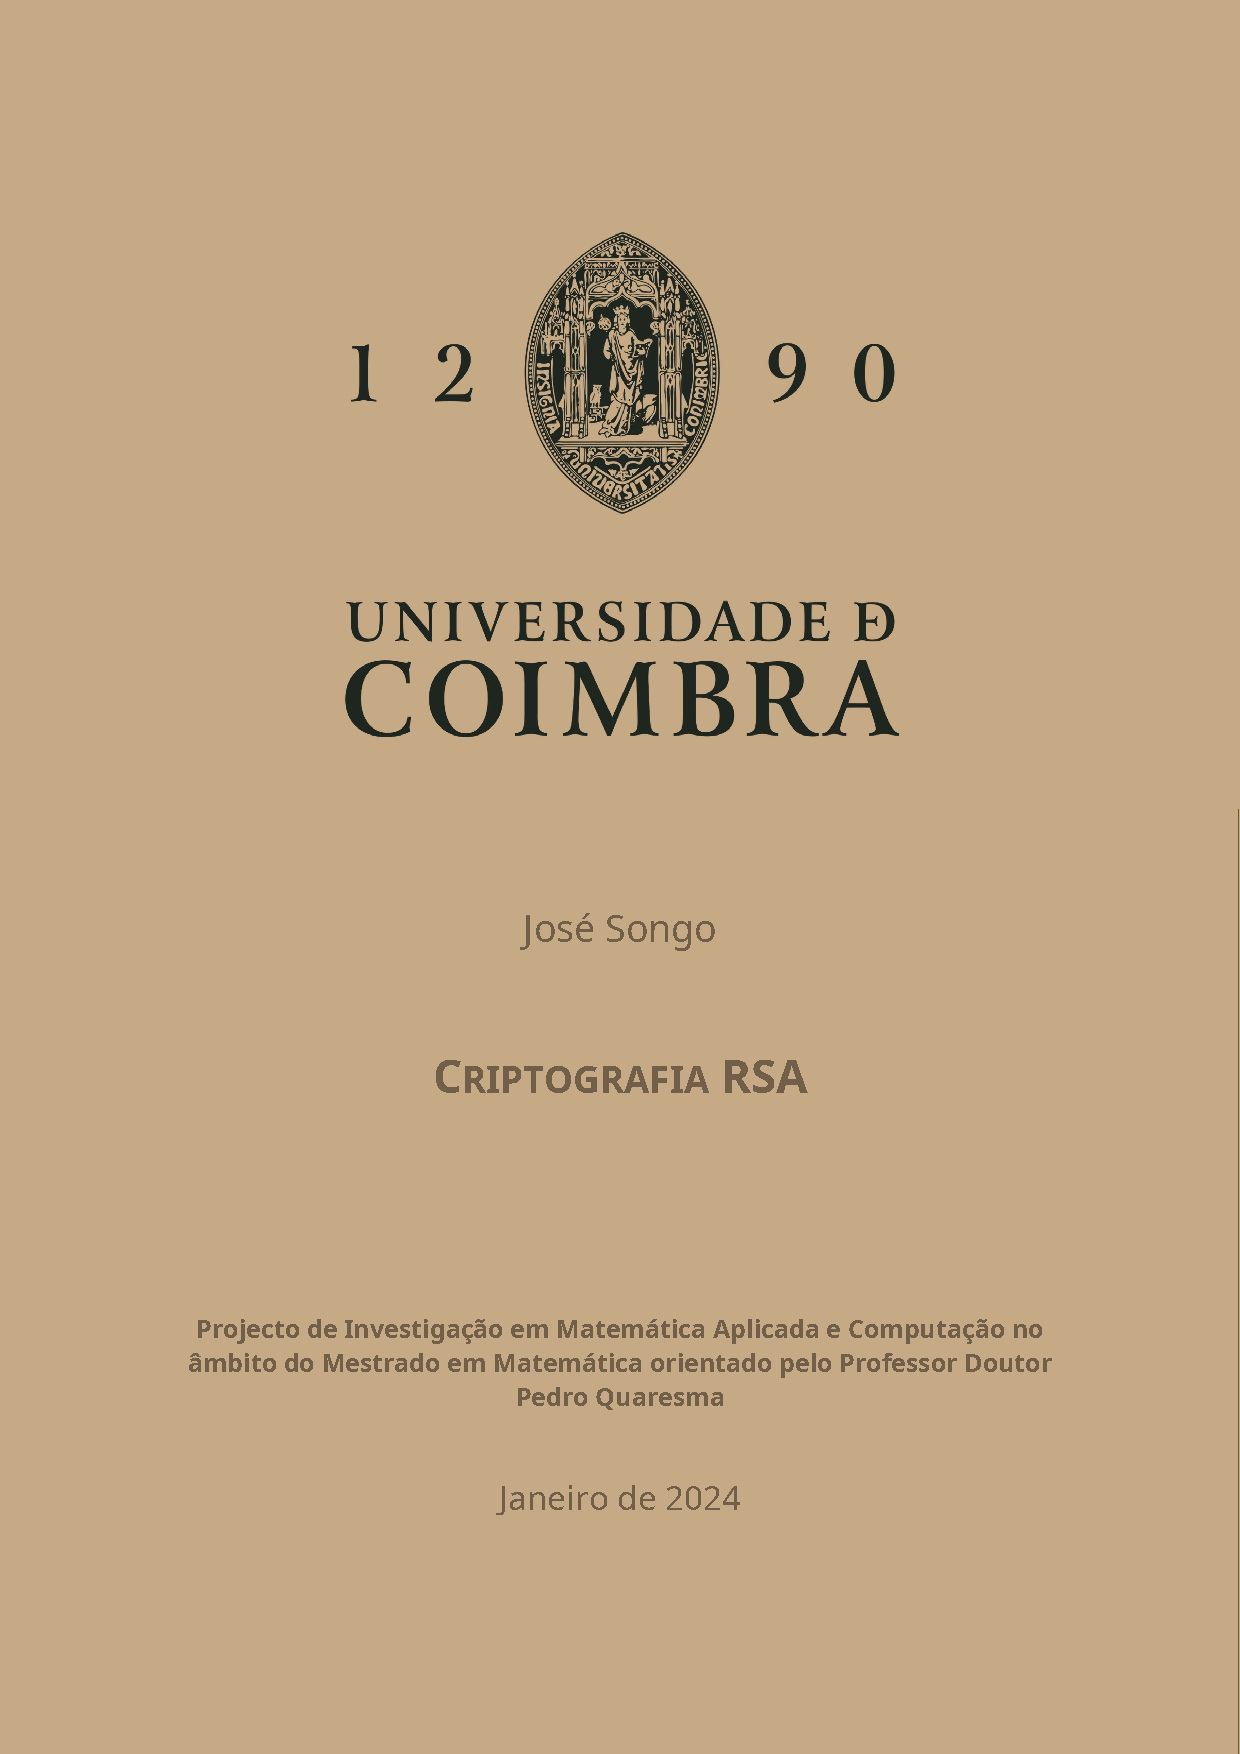
\includepdf{Cover/Capa_Dissertacao_TPL-A4.pdf}


\frontmatter

\begin{titlepage}
  \vspace*{30mm}
  \maketitle
\end{titlepage}


% ************************** Thesis Acknowledgements *****************************

\begin{acknowledgements}


Agradeço ao professor Pedro Quaresma, que aceitou orientar o meu projeto, revelando uma especial atenção às minhas ideias. Os seus conselhos e sugestões bem como a valorização do trabalho desenvolvido foram determinantes para alcançar este resultado.


\end{acknowledgements}

% ************************** Thesis Abstract *****************************
% Use `abstract' as an option in the document class to print only the titlepage and the abstract.
\begin{abstract}
\ifisLangEn

If the Dissertation is in Portuguese, do not write here anything.
This is where you write your abstract in English.

% ************************************************************************
%
% As linhas seguintes definem o `resumo' em portugu\^{e}s apenas no caso
% da l\'{\i}ngua utilizada ser o ingl\^{e}s. Caso contr\'{a}rio, ser\~{a}o ignoradas.
%
% ************************************************************************

  \cleardoublepage
  \setsinglecolumn
  \chapter*{\centering \Large Resumo}
  \thispagestyle{empty}

\else
  %Aqui escreve o Resumo em Portugu\^{e}s no caso da disserta\c{c}\~{a}o usar o Ingl\^{e}s.

    A criptografia RSA revolucionou a segurança digital com o seu procedimento de chaves pública e privada, em contraponto com as cifras de chaves simétricas cuja gestão das chaves é muito difícil de gerir em ambientes com muitos intervenientes. A criptoanálise, por sua vez, desempenha um papel fundamental na avaliação e no aprimoramento da segurança dos sistemas criptográficos, buscando constantemente formas de tornar as comunicações digitais mais seguras e protegidas contra ameaças cibernéticas.

    Neste texto apresentam-se as implementações dos diferentes métodos descritos no trabalho de seminário, nomeadamente, os algoritmos para os métodos de deslocamento simples, linear e RSA.
    
    No final, foi feito um estudo comparativo dos métodos acima mencionados.
\fi
\end{abstract}


% *********************** Adding TOC and List of Figures ***********************

\tableofcontents

%\listoffigures

\listoftables

\lstlistoflistings

% *********************** Index of Nomenclature (Optional) ***********************
%
%% printnomencl should be commented out, if you are using a list of Nomenclature
%
% ********************************************************************************

%% In case you don’t like the name of the nomenclature, just redefine the \nomname macro, e. g.
%\renewcommand{\nomname}{List of symbols}

%\printnomencl

%% It uses the package nomencl
%%\printnomencl[space] space can be set as 2em between symbol and description
%%\printnomencl[3em]

%%%% IMPORTANT: The nomencl package only creates a fyle thesis.nlo.
%%%%            You need to create the file thesis.nls that contains your nomenclature list properly ordered.
%%
%% In order to do that and to include the list in the pdf the compile sequence must be:
%% run pdfLaTeX
%% run makeindex thesis.nlo -s nomencl.ist -o thesis.nls
%% then rerun pdfLaTeX


% ******************************** Main Matter *********************************
\mainmatter

%*******************************************************************************
%*********************************** First Chapter *****************************
%*******************************************************************************


\chapter{Introdução}


A criptografia é uma técnica antiga e importante utilizada para proteger informações confidenciais por meio da codificação e descodificação de mensagens. Ela desempenha um papel essencial na segurança da comunicação, impossibilitando que terceiros não autorizados compreendam ou acessem o conteúdo das mensagens.~\cite{Quaresma2008a,Quaresma2009a}.

Um dos exemplos mais simples de criptografia é a cifra de Júlio César, também conhecida como cifra de deslocamento ou cifra de substituição. Essa técnica foi usada pelo renomado imperador romano Júlio César (100aC -- 44aC) para enviar mensagens secretas durante as suas ações militares.

A cifra de Júlio César funciona substituindo cada letra do alfabeto por outra, deslocando um número fixo de posições para a esquerda ou direita no alfabeto. Por exemplo, se usarmos um deslocamento de 3 posições para a direita, a letra ``a'' seria substituída pela letra ``d'', ''b'' seria substituída por ``e'', e assim por diante. Ao chegar ao fim do alfabeto, volta-se ao início, por exemplo ``x'' passa a ``a'',``y'' passa a ``b'' e ``z'' passa a ``c''.

Essa técnica simples demonstra os princípios fundamentais da criptografia, onde a informação original é escondida de uma maneira específica para ocultar seu significado, e somente aqueles que possuem a chave podem decifrar a mensagem.

No entanto, a cifra de Júlio César é bastante vulnerável a ataques de força bruta, pois há um número limitado de combinações possíveis. Por isso, ela é considerada uma forma trivial de criptografia e não é adequada para proteger informações sensíveis nos dias atuais. Hoje em dia, algoritmos mais complexos e seguros são utilizados para garantir a segurança das comunicações, como AES (Advanced Encryption Standard) e RSA (Rivest-Shamir-Adleman), oferecendo níveis avançados de proteção.
\chapter{Criptografia Clássica}

Designa-se usualmente por \emph{criptografia clássica} as cifras  pré-computacionais, desenvolvidas e utilizadas tendo por base processos mecânicos ou manuais. O mais simples deste tipo de criptografia consiste em trocar uma letra pela seguinte. Um código similar foi usado por Júlio César, cuja a chave era estabelecida pelo deslocamento, de três posições, nas letras do alfabeto~\cite{Coutinho2005}.

\begin{definicao}[Cifra Deslocamento]
 Seja $\mathcal{M}=\mathcal{C}=\mathbb{Z}_{26}^*$, $\mathcal{K}=\mathbb{Z}_{26}$. 7
 Para $0 \leq K \leq \mid\mathbb{Z}_{26}\mid$=26, define-se:
$$e_k(x)=(x+K) \; mod \; 26$$ e $$d_k(y)=(y - K) \; mod \; 26$$ para todo o $x,y \in \mathbb{Z}_{26}$
\end{definicao}

\emph{Nota:} para $\mathbb{Z}_{n}$ tem-se $n=26$ uma vez que o alfabeto adotado tem 26 caracteres.

\begin{teorema}[Cifra Deslocamento Simples] As funções $e_k$ e $d_k$ constituem uma cifra.
\end{teorema}
\begin{demonstracao}
    \begin{align*}
    d_k(e_k(x)&=d_k(x+k)=\\
              &=(x+k)-k=\\
              &=x\;mod\;26
\end{align*}

Então, por definição,a cifra de deslocamento é uma cifra.
\end{demonstracao}


\begin{definicao}[Cifra Deslocamento Linear]
    Seja $\mathcal{M}=\mathcal{C}=\mathbb{Z}_{26}^*$, e seja:
$K=\{(a,b) \in \mathbb{Z}\times \mathbb{Z} : mdc(a,26)=1\}$.

Para $K=(a,b) \in \mathcal{K}$, define-se:
$$ e_k(x)=(ax + b)\;mod\;26$$
e
$$ d_k(y)=a^{-1}(y - b)\;mod\;26$$
para todo o $x,y \in \mathbb{Z}_{26}$
\end{definicao}

\begin{teorema}[Cifra deslocamento linear] As funções $e_k$ e $d_k$ constituem uma cifra.
\end{teorema}
\begin{demonstracao}
    \begin{eqnarray*}
    d_k(e_k(x)) & = & d_k(ax +b)\\
                & = & a^{-1}(ax+b -b)\quad\text{\;por definição $a$ é invertível em $\mathbb{Z}_{26}$}\\
                & = & a^{-1}ax\\
                & = & x
    \end{eqnarray*} 
Por definição, verifica-se que o resultado apresentado anteriormente é verdadeiro.
\end{demonstracao}


Relativamente à criptoanálise, as cifras clássicas são cifras muito fracas ou completamente inseguras pelo que estão suscetíveis a ataques por procura exaustiva. Também é possível quebrar esta cifra por ataques baseada na frequência relativa das letras, diagramas,trigramas, letras iniciais e finais das palavras.

Por exemplo, se todas as todas as ocorrências da letra $a$ são substituídas pela letra $x$, uma mensagem cifrada contendo muitas instâncias da letra $x$, iria sugerir ao criptoanalista, que a letra $x$ representa a letra $a$.

De facto, para uma dada linguagem verifica-se que cada letra aparece de acordo com uma frequência própria. No caso da língua portuguesa tem-se a seguinte tabela de frequência:~\cite{Quaresma2009a}:

\begin{table}[h]
\centering
\begin{tabular}{>{\columncolor{gray!20}}cccccccccc}
a & 12,71\% & \cellcolor{gray!20}b & 0.81\% & \cellcolor{gray!20}c & 4,16\% & \cellcolor{gray!20}d  & 5,52\% & \cellcolor{gray!20}e & 11,99\% \\
f & 1,43\% & \cellcolor{gray!20}g & 1,32\% & \cellcolor{gray!20}h & 0,74\% & \cellcolor{gray!20}i  & 7,18\% & \cellcolor{gray!20}j & 0,21\% \\
k & 0,00\% & \cellcolor{gray!20}l & 3,23\% & \cellcolor{gray!20}m & 4,48\% & \cellcolor{gray!20}n  & 5,24\% & \cellcolor{gray!20}o & 11,32\% \\
p & 3,07\% & \cellcolor{gray!20}q & 1,41\% & \cellcolor{gray!20}r & 6,47\% & \cellcolor{gray!20}s  & 7,99\% & \cellcolor{gray!20}t & 5,31\% \\
u & 3,44\%  & \cellcolor{gray!20}v & 1,36\% & \cellcolor{gray!20}w & 0.02\% & \cellcolor{gray!20}x  & 0,28\% & \cellcolor{gray!20}y & 0,02\% \\
z & 0,37\% & & & & & &  & & \\
\end{tabular}
\end{table}

Com estes dados, agrupa-se estes valores em grupos, das letras com maior frequência para as menos frequentes:

\begin{table}[h]
\centering
\begin{tabular}{>{\columncolor{gray!20}}ccccc}
Primeiro grupo  & \cellcolor{gray!20}Segundo grupo & \cellcolor{gray!20}Terceiro grupo & \cellcolor{gray!20}Quarto grupo  & \cellcolor{gray!20}Quinto grupo\\
a,e,o &s,r,i & n,d,m,u,t,c &  l,p,v,g,h,q,b,f  & z,j,x,k,w,y\\
\end{tabular}
\end{table}

Notar que este processo reduz o número de tentativas e erro a realizar antes de se conseguir quebrar o código tornando-o mais eficiente.

Logo para quebrar a cifra utilizada para obter o texto encriptado ``a fkdyh whp gh vhu pdqwlgd', sabendo que foi utilizado um sistema de cifração de deslocamento simples, precisamos de calcular as frequências relativas para o texto cifrado,tem-se:


\begin{table}[h]
\centering
\begin{tabular}{>{\columncolor{gray!20}}cccccccccc}
d & 17,9\% & \cellcolor{gray!20}f & 7,1\% & \cellcolor{gray!20}g & 7,1\% & \cellcolor{gray!20}h & 21,4\% \\
k & 3,6\% & \cellcolor{gray!20}l & 3,6\% & \cellcolor{gray!20}p & 7,1\% & \cellcolor{gray!20}q & 3,6\% \\
u & 7,1\% & \cellcolor{gray!20}v & 7,1\% & \cellcolor{gray!20}w & 10,7\% & \cellcolor{gray!20}y & 3,6\% \\
\end{tabular}
\end{table}
Por análise das frequências relativas e consultado o primeiro grupo, onde as letras tem maior frequência relativa, uma vez que ``d'', com $17,9\%$, e o ``h'', com $21,4\%$ então podemos fazer ``d'' corresponder a ``a'', por exemplo. Neste caso, a nossa chave é 3.

Assim, obtemos o texto claro ``a chave tem de ser mantida secreta''. Logo a cifra foi quebrada.~\cite{Quaresma2009a}

Com recurso do computador podemos facilmente realizar todo o processo anterior rapidamente pelo que este tipo de cifra é muito fraca.

\chapter{Criptografia RSA}
\label{sec:criptografiaRSA}

A implementação do algoritmo RSA é bastante utilizado para assegurar a segurança das comunicações digitais. Este algoritmo baseia-se em um par de chaves: uma chave pública utilizada para encriptar os dados e uma chave privada correspondente para desencriptar.

Na encriptação RSA, o remetente utiliza a chave pública do destinatário para transformar os dados originais em um formato encriptado. O resultado é um texto encriptado, que pode ser enviado com segurança.

Por outro lado, na desencriptação RSA, o destinatário utiliza sua chave privada correspondente para reverter o processo anterior. Com isso, o destinatário obtém novamente os dados originais, protegendo a confidencialidade da informação.

A segurança do algoritmo RSA baseia-se na dificuldade de fatorizar números primos de grande dimensão, pois as chaves pública e privada são geradas a partir desses números.\footnote{Size considerations for public and private keys, \url{https://www.ibm.com/docs/en/zos/2.3.0?topic=certificates-size-considerations-public-private-keys}}

Portanto, uma implementação bem-sucedida da cifra RSA requer desenvolver corretamente algoritmos matemáticos, incluindo geração de chaves, encriptação e  desencriptação garantindo assim a segurança das comunicações digitais. Também são criadas funções secundárias que auxiliam as funções mencionadas anteriormente, nomeadamente de conversão e de operação de congruência.

\section{Cifra RSA---Geração das Chaves}
\label{ec:cifraRSAGeracaoChaves}
Para empregar o algoritmo RSA, em primeiro lugar,  é preciso gerar chaves pública e privada para cifrar ou decifrar a mensagem, respetivamente.  

Seja $(e,n)$ a chave pública e $(d,n)$ a chave privada, onde \emph{e} tal que $1<e<\phi(n)$ é primo relativo com $\phi(n)$ e \emph{d} é o inverso multiplicativo de \emph{e} módulo $\varphi(n)$, ou seja $de \equiv 1(mod \phi(n))$.

\begin{itemize}
    \item[$\hookrightarrow$] \emph{p}, \emph{q}, dois números primos de grande dimensão;
    \item[$\hookleftarrow$] \emph{(e,n)} e \emph{(d,n)}, as chaves: pública e privada
\end{itemize}
\begin{lstlisting}[frame=single,mathescape=true,caption={Cifra RSA ---Especificação de \texttt{GerarChavePrivada}},captionpos=b,label={lst:gerarChavePrivada},basicstyle=\footnotesize]
int* gerarChavePrivada(int , int ,int );
\end{lstlisting}
\begin{lstlisting}[frame=single,mathescape=true,caption={Gerar chave privada},captionpos=b,label={lst:Gerar chave privada},basicstyle=\footnotesize]
int* gerarChavePrivada(int p, int q,int e){
// Aloca dinamicamente um array de 2 inteiros
    int* chaveP = (int*)malloc(2 * sizeof(int)); 

if (chaveP == NULL) {
    // Se a alocação falhar
    return NULL;
}
chaveP[0]=inversoMultiplicativo((p-1)*(q-1),e);
chaveP[1]=p*q;
return chaveP;
}
\end{lstlisting}
\begin{lstlisting}[frame=single,mathescape=true,caption={Cifra RSA ---Especificação de \texttt{GerarChavePública}},captionpos=b,label={lst:gerarChavePublica},basicstyle=\footnotesize]
int* gerarChavePublica(int ,int );
\end{lstlisting}
\begin{lstlisting}[frame=single,mathescape=true,caption={Gerar chave privada},captionpos=b,label={lst:Gerar chave privada},basicstyle=\footnotesize]
int* gerarChavePublica(int q,int p){
// Aloca dinamicamente um array de 2 inteiros
int* chaveP = (int*)malloc(2 * sizeof(int)); 
int omega_n=(p-1)*(q-1);
if (chaveP == NULL) {
    // Se a alocação falhar
    return NULL;}
//chaveP[1]=(p-1)*(q-1);
chaveP[1]=p*q;
//calcular e -->pequeno para melhorar a encriptação
for(int i=2;i<omega_n;i++){
    
    if(ePrimo(i,omega_n)){
        chaveP[0]=i;
        break;}}
    return chaveP;}
\end{lstlisting}


\section{Cifra RSA---Encriptação}
\label{ec:cifraRSAencriptacao}

Para a encriptação RSA tem-se:

\begin{itemize}
    \item[$\hookrightarrow$] mensagem a cifrar, a chave pública, $(e,n)$;
    \item[] encriptar número a número através da função de encriptação;
    \item [$\hookleftarrow$] texto cifrado.
\end{itemize}

\begin{lstlisting}[frame=single,mathescape=true,caption={Cifra RSA ---Especificação de \texttt{CifraEncriptar}},captionpos=b,label={lst:rsaCifraEncriptar},basicstyle=\footnotesize]
int cifraEncriptar(int,int,int);
\end{lstlisting}

\begin{lstlisting}[frame=single,mathescape=true,caption={Encriptação RSA},captionpos=b,label={lst:EncriptacaoRSA},basicstyle=\footnotesize]
void encriptar(int e,int n,fstream& fin,fstream& fout){
int i=0,aux;
string linha;
string nomeMsg;
while (getline(fin, linha)) {//Obter as linhas do ficheiros
      while(linha[i]!='\0'){
        //converter as letras da linha em numeros
        aux=conversaoDS_LN(linha[i]);
        aux=cifraEncriptar(e,n,aux);//Aplicação de encriptação
        i+=1;
        if(aux > n){
            aux=aux%(n);}
        fout <<aux<<" ";}
    fout << endl;
    i=0;}
fout.close();//fechar ambos os ficheiros
fin.close();}

\end{lstlisting}

\section{Cifra RSA---Desencriptação}
\label{ec:cifraRSAdesencriptacao}


Ao receber um texto cifrado, o destinatário precisa seguir um conjunto de passos para obter a mensagem original. O processo de desencriptação inicia-se com a mensagem a ser decifrada, que foi previamente cifrada usando a chave pública correspondente. A chave de desencriptação, mantida em segredo pelo destinatário, é indispensável para este procedimento.

Portanto a geração da chave de desencriptação é um passo essencial, pois é por meio dela que a informação codificada pode ser revertida ao seu estado original. Esta chave, em conjunto com a função de desencriptação associada ao algoritmo RSA, permite o processo de decifração do texto original.

Logo ao desencriptar número a número através da função de desencriptação utilizando a chave privada correspondente, o destinatário é capaz de recuperar o texto original, assegurando a privacidade e a segurança das informações transmitidas. 

Portanto para desencriptação RSA tem-se:
\begin{itemize}
    \item[$\hookrightarrow$] mensagem a decifrar;
    \item[] desencriptar número a número através da função de desencriptação;
    \item [$\hookleftarrow$] texto original.
\end{itemize}

\begin{lstlisting}[frame=single,mathescape=true,caption={Cifra RSA ---Especificação de \texttt{CifraDesencriptar}},captionpos=b,label={lst:rsacifraDesencriptar},basicstyle=\footnotesize]
void desencriptar(int,int ,fstream& ,fstream& );
\end{lstlisting}

\begin{lstlisting}[frame=single,mathescape=true,caption={Gerar chave privada},captionpos=b,label={lst:Gerar chave privada},basicstyle=\footnotesize]
void desencriptar(int p,int q,fstream& fin,fstream& fout){
int i=0,aux,d;
int* chaveP = (int*)malloc(2 * sizeof(int)); // Aloca dinamicamente array
if (chaveP == NULL){
    // Se a alocação falhar
    cout<<"Alocação falhou...";}
chaveP=gerarChavePublica(p,q);
d=inversoMultiplicativo(chaveP[1],chaveP[0]);
string nomeMsg;
string linha;
    while (getline(fin, linha)) {//Obter as linhas do ficheiros
          istringstream linhaAux(linha);
          while(linhaAux >> aux){
          //Aplicação de encriptação
          aux=cifraEncriptar(d,p*q,aux);
            i+=1;
            if(aux > (p*q)){
                aux=aux%(p*q);}
            fout << conversaoDS_NL(aux);}
        fout << endl;
        i=0;}
    //fechar ambos os ficheiros
    fin.close();fout.close();}
\end{lstlisting}
%%% Local Variables:
%%% mode: latex
%%% TeX-master: "../thesis"
%%% End:


\chapter{Criptoanálise RSA}
\label{sec:CriptoanaliseRSA}

O sistema RSA é assimétrico, ou seja, possui uma chave pública $(e,n)$ e uma chave privada $(d,n)$, em que~\cite{Quaresma2009a}:

\begin{itemize}
    \item[]$n=p \times q$ com $p$ e $q$ números primos;
    \item[]$1<e< \phi(n)$, em que $\phi(n)$, a funçao de Euler, é igual ao número co-primos de $n$;
    \item[]$de\equiv 1(mod\phi(n))$
\end{itemize}

Sabemos que a chave pública é $(e,n)$, portanto apenas tem-se que fatorizar $n$ no produto de números primos $p$ e $q$ para obtermos $d$ e, com isso, a chave secreta $(d,n)$. No entanto, fatorizar um número em fatores primos é um problema computacionalmente difícil~\cite{Quaresma2009a}.

Para a implementação dos algoritmos a seguir optou-se pelo tipos de dados ``\emph{unsigned long long int}'' uma vez que apenas iremos lhe dar com números positivos de grande dimensão.


\section{Método da Divisão}
\label{sec:MetodoDivisao}

Sendo um método de força bruta, vai-se tentar a divisão sucessiva por todos os números primos até $\lfloor \sqrt{n} \rfloor$ , ou até que a solução seja encontrada.

\begin{lstlisting}[frame=single,mathescape=true,caption={Criptoanálise RSA ---Especificação de \texttt{MétodoDivisao}},captionpos=b,label={lst:metodoEuclides},basicstyle=\footnotesize]
unsigned long long int  metodoDivisao(unsigned long long int  );
\end{lstlisting}

\begin{lstlisting}[frame=single,mathescape=true,caption={Método de Divisão},captionpos=b,label={lst:MetodoDivisao},basicstyle=\footnotesize]
unsigned long long int  metodoDivisao(unsigned long long int  n){	
unsigned long long int  *resCrivo = new unsigned long long int [n + 1],i;
crivo(n,resCrivo);//Determinar os números primos
for(i=2;i<=n;i++){
    if(resCrivo[i]){//verificar quais dos numeros sao primos
        if((n%i)==0){
            return i;//retornar numero primo
        }
    }
 }
 return 0;
}
\end{lstlisting}

Primeiramente, é necessário utilizar um método que elabore a lista de todos os números primos até um limite definido, e neste caso, foi utilizado o Crivo de Eratóstenes.

\emph{Crivo de Eratóstenes}
\begin{itemize}
    \item[] começa-se por gerar um vetor com todos os números de 2 até $n$;
    \item[]2 é primo;
    \item[]Então utiliza-se o 2 para retirar todos os seus multiplos da lista, e assim sucessivamente;
    \item[]os elementos que restar após as sucessivas aplicações constituem os números primos de 2 até $n$.
\end{itemize}
A necessidade de gerar a lista completa de todos os inteiros de 2 até $n$ e iterar sobre ela várias vezes, pois é necessário percorrer essa lista para aplicar os sucessivos crivos, leva a que a utilização do \emph{crivo de Erastóstenes} acrescente um peso muito significativo ao algoritmo, tanto temporal como especialmente~\cite{Quaresma2009a}.

\section{Método de Euclides}
\label{sec:MetodoEuclides}

Este algoritmo consiste em multiplicar todos os números entre 2 e $\lfloor \sqrt{n} \rfloor$, calcular de seguida o \emph{mdc} entre esse produto e \emph{n}, de forma a encontrar o fator primo pretendido.

Para evitar o problema de representação computacional dos números que se obtém do produto dos números primos de grande dimensão, vai dividir-se a multiplicação em vários produtos parcelares.

Para tal, os passos seguintes são adotados:

\begin{itemize}
    \item Começa-se por definir os conjuntos auxiliares:

    $R={r_1,r_2,\dots,r_n}$, representando $r_i$ um limite inferior $(r_1=1,\;r_i<r_{i+1});$
    
    $S={s_1,s_2,\dots,s_n}$, representando $s_i$ um limite superior$(s_i<s{i+1},s_{m-1}<\lfloor \sqrt{n} \rfloor<s_m)$;
    \item Para cada par $r_i$ e $s_i$, multiplicam-se todos os números primos entre estes dois limites, $P_i=\prod_{r_i\leq p_i \leq s_i}p_i$;
    \item Para cada um dos $P_i$ calcula-se o $mdc(P-i,n)=a_i$;
    \item Se $a_i \neq 1 $, então $a_i$ é o factor primo de $n$ que se pretende obter~\cite{Quaresma2009a}.
\end{itemize}

\begin{lstlisting}[frame=single,mathescape=true,caption={Criptoanálise RSA ---Especificação de \texttt{MétodoEuclides}},captionpos=b,label={lst:metodoEuclides},basicstyle=\footnotesize]
unsigned long long int  metodoEuclides(unsigned long long int  );
\end{lstlisting}

\begin{lstlisting}[frame=single,mathescape=true,caption={Método de Euclides},captionpos=b,label={lst:MetodoEuclides},basicstyle=\footnotesize]
unsigned long long int  metodoEuclides(unsigned long long int  n){
unsigned long long int  *resCrivo = new unsigned long long int [n + 1],
i,aux,lim,res=1;
aux=floor(sqrt(n));
lim=(aux/10)+1;
unsigned long long int  *resM= new unsigned long long int [aux+1];
for(i=0;i<=lim;i++){
    resM[i]=1;
    }
crivo(n,resCrivo);//encontrar os numeros primos
for(i=2;i<=aux;i++){
    if(resCrivo[i]){
        resM[(i/10)]=i*resM[i/10];//calcular o produto
    }
}
i=0;
while(i<lim){
    if(mdc(resM[i],n)> 1){//verifcar mdc(resM[i],n]
        return mdc(resM[i],n);
    }		
    i++;
}
delete[] resCrivo;
delete[] resM;
return res;
}
\end{lstlisting}

Mais uma vez, tivemos de gerar números primos até $n$ que é pesado temporalmente. Além disso, apenas atenuamos o problema anterior quando fizemos a multiplicação parcelar para contornar o obstáculo de representação computacional relativamente ao resultado da  multiplicação dos números primos uma vez que à medida que $n$ aumentar voltaremos a ter o mesmo problema.

\section{Método de Fermat}
\label{sec:MetodoFermat}

Este método consiste em obter dois inteiros $a$ e $b$ que permitam representar o número natural $n$ como a diferença de dois quadrados~\cite{Quaresma2009a}.

Para determinar os inteiros $a$ e $b$ de forma que $n=a^2 - b^2$, o processo pode ser conduzido da seguinte maneira:
\begin{itemize}
    \item[] Dado um inteiro $n$ ímpar começamos por $a=\lfloor \sqrt{n} \rfloor +1$
    \item[] Se $b=\sqrt{a^2-n}$ é um inteiro, obtém-se o pretendido
    \item[] Caso contrário, incrementamos a de uma unidade até que b seja um inteiro;
\end{itemize}


\begin{lstlisting}[frame=single,mathescape=true,caption={Criptoanálise RSA ---Especificação de \texttt{MétodoFermat}},captionpos=b,label={lst:metodoFermat},basicstyle=\footnotesize]
unsigned long long int* metodoFermat(unsigned long long int );
\end{lstlisting}

\begin{lstlisting}[frame=single,mathescape=true,caption={Método de Fermat},captionpos=b,label={lst:MetodoFermat},basicstyle=\footnotesize]
unsigned long long int* metodoFermat(unsigned long long int n){
long double a,b;
unsigned long long int *res= new unsigned long long int[2];
a=floor(sqrt(n))+1;
b=sqrt(a*a-n);
//retorna o maior número inteiro menor ou n
while(abs(b - floor(b)) > std::numeric_limits<long double>::epsilon()){
a=a+1;//incrementar a
b=sqrt(a*a-n);//incrementar b
}
//calcular p e q
res[0]=a+b;
res[1]=a-b;
return res;
}
\end{lstlisting}
Como veremos mais a frente, este método mostra que quanto maior a diferença entre \emph{p} e \emph{q} maior vai ser o número de tentativas precisas para obter um valor inteiro para a raiz.

\section{Estudo Comparativo dos Métodos}
Os dados foram obtidos a partir de testes realizados em um ambiente computacional, utilizando o sistema Windows 10 Home, processador Intel(R) Core(TM) i3-7020U CPU 2.30GHz e memória RAM de 4 GB. 
Pode-se afirmar que, se a seleção dos números primos for apropriada, a segurança da cifra RSA é mantida.

\begin{table}[h]
\centering
\caption{Estudo comparativo dos métodos}
\label{tab:EstudoMetodo}
\begin{tabular}{>{\columncolor{gray!20}}ccccc}
n & \cellcolor{gray!20}Fatores & \cellcolor{gray!20}Divisão & \cellcolor{gray!20}Euclides & \cellcolor{gray!20}Fermat\\
$1457$ & $p=31$, $q=47$ & $0,\!000s$ &$0,\!000s$&$0,\!000s$\\
13199 &$p=67$, $q=197$&$0,\!002s$ & $0,\!002s$& $$0,\!000s$$\\
$281161$ & $p=79$, $q=3559$  & $0,\!136s$& $0,\!145s$&$0,\!000s$\\
$701123$ & $p=3559$, $q=197$ &$0,\!521$s& $0,\!482s$&$0,\!003s$\\
$23420707$&$p=41017$, $q=571$ & $71,124s$ & $64,86s$&$0,\!000s$\\
$488754769$ & $p=110503$, $q=4423$  & $-$ & $-$&$0,005s$\\
$2027651281$ & $p=46061$, $q=41017$ & $-$ & $-$&$0,\!000s$\\
$103955963689$ & $p=47188363$, $q=2203$  & $-$& $-$&$1,75s$\\
$210528952589$ & $p=95564663$, $q=2203$  & $-$ & $-$&$3,635s$\\
$2746662891777043$ & $p=47188363$, $q=58206361$  & $-$ & $-$&$0,024s$\\
$4509540007616669$ & $p=47188363$, $q=95564663$  & $-$ & $-$&$0,299s$\\
\end{tabular}
\end{table}


Com efeito, por observação da tabela \emph{Estudo comparativo dos métodos} constata-se que:

\begin{itemize}
    \item[] Os métodos de Divisão e Euclides apresentam um aumento considerável no tempo de execução à medida que os fatores primos crescem significativamente, além de perderem eficácia na resolução do problema mesmo para valores relativamente pequenos de $n=p\times q$. Essas limitações surgem da exigência de gerar números primos até $\lfloor \sqrt{n} \rfloor$ e, no caso do método de Euclides, da multiplicação de números de grande escala.
    \item[]O método de Fermat observa um aumento muito acentuado em seus tempos de execução com o crescimento da dimensão dos fatores primos; no entanto, uma análise mais detalhada revela que quando os fatores primos estão em proximidade, o método de Fermat demonstra ser altamente eficaz.
\end{itemize}

Podemos inferir que, para garantir a segurança da criptografia RSA contra os métodos apresentados acima, os fatores primos devem estar consideravelmente distantes um do outro, e o valor de $n$ deve ser maior que 20 dígitos decimais~\cite{Quaresma2009a}.

Presentemente, sobretudo devido a algoritmo mais eficazes, a cifra RSA utiliza valores de $n$ com 1024 bits (a que corresponde 309 dígitos decimais) ou mais~\cite{Quaresma2009a}.\footnotemark[1]


%\textcolor{red}{PQ: \url{https://en.wikipedia.org/wiki/RSA_Factoring_Challenge} }

%%% Local Variables:
%%% mode: latex
%%% TeX-master: "../thesis"
%%% End:

\chapter{Conclusões}
\label{sec:Conclusoes}
Ao longo do trabalho constatou-se o procedimento eficaz e seguro para criptografar a informação desempenhada  pela sistema RSA.

De facto, verifica-se na secção~\ref{sec:CriptoanaliseRSA} que os métodos analisados não têm capacidade de ``quebrar'' o método RSA em chaves maiores que 20 dígitos. As chaves seguras utilizadas atualmente para o algoritmo RSA têm cerca de 2048 bits.\footnote{Ver página: \emph{Size considerations for public and private keys}, \url{https://www.ibm.com/docs/en/zos/2.3.0?topic=certificates-size-considerations-public-private-keys}}

No próximo semestre, iremos aprofundar o estudo da criptoanálise do método RSA, com foco especial no crivo quadrático."



%%% Local Variables:
%%% mode: latex
%%% TeX-master: "../thesis"
%%% End:

%\include{Chapter6/chapter6}
%\include{Chapter7/chapter7}



% ********************************** Back Matter *******************************
%% Backmatter should be commented out, if you are using appendices after References

%\backmatter

% ********************************** Bibliography ******************************
\begin{spacing}{0.9}

% To use the conventional natbib style referencing
% Bibliography style previews: http://nodonn.tipido.net/bibstyle.php
% Reference styles: http://sites.stat.psu.edu/~surajit/present/bib.htm

\bibliographystyle{apalike}
%\bibliographystyle{plainnat} % use this to have URLs listed in References
\cleardoublepage
\bibliography{References/references} % Path to your References.bib file


% If you would like to use BibLaTeX for your references, pass `custombib' as
% an option in the document class. The location of 'reference.bib' should be
% specified in the preamble.tex file in the custombib section.
% Comment out the lines related to natbib above and uncomment the following line.

%\printbibliography[heading=bibintoc, title={References}]


\end{spacing}

% ********************************** Appendices ********************************

% *************************************** General Index ********************************
%\printthesisindex % If index is present


\end{document}

%%% Local Variables:
%%% mode: latex
%%% TeX-master: t
%%% End:
